% The Vector Is the Product — main paper (arXiv preprint).
% Ported from draft.md (2026-08-11). Numbers: RESULTS.md (Ext 8–17).
% Tables are the canonical ones from main_tables.tex (kept in sync).
% Build: tectonic paper/paper.tex
\documentclass[10pt,twocolumn]{article}
\usepackage[margin=0.85in]{geometry}
\usepackage{booktabs}
\usepackage{multirow}
\usepackage{graphicx}
\usepackage{amsmath}
\usepackage{amssymb}
\usepackage{caption}
\usepackage{newtxtext}
\usepackage[dvipsnames]{xcolor}
\usepackage{hyperref}
\captionsetup{font=small,labelfont=bf}
\hypersetup{colorlinks=true,linkcolor=black,citecolor=NavyBlue,urlcolor=NavyBlue}

\newcommand{\sd}[1]{\textbf{#1}}
\newcommand{\pstar}{$^{*}$}
\newcommand{\pstarstar}{$^{**}$}
\newcommand{\pstarstarstar}{$^{***}$}
\newcommand{\head}{readout}
\newcommand{\loopk}{loop.$k$}

\title{\textbf{The Vector Is the Product:\\
One-Pass Readouts of Frozen Language-Model Residuals\\
Match the Autoregressive Loop}}
\author{}
\date{}

\begin{document}
\maketitle

\begin{abstract}
On tasks whose answer is representable in a single forward pass, the
autoregressive loop is not the only readout of a language model's computation
--- and, we show, not a privileged one. We fit small supervised heads to the
frozen final-token residual of six open-weight models (Qwen3-0.6B/4B/8B,
Mistral-7B, Granite-3.1-8B, DeepSeek-V4-Flash) and run the \head{}
head-to-head against a fairly-conditioned autoregressive loop --- full
context, balanced few-shot, scored by next-token log-probability over the
answer set --- matched on information access, scoring protocol, and
supervision budget. On BoolQ (full validation), RuleTaker (n2k), and
ARC-Challenge (full test), the one-pass \head{} \textbf{matches or beats} the
fair loop at nearly every scale: it wins significantly where the model is
weakest (RuleTaker $+9.3$pt at 0.6B, $+13.3$pt on Granite-8B; BoolQ $+3.8$pt
at 0.6B against a $4\times$-budget loop), ties at mid scale, and loses
decisively only in two regimes --- small models on parametric knowledge (ARC)
and a frontier MoE on serial deduction. The result survives label-shuffle
nulls, random-projection selectivity, per-length deconfounds, and paired
significance testing on identical rows. Sweeping the \head{} tap across
depth, the verdict representation is fully assembled by mid-depth: the best
mid-layer tap beats the final layer significantly at 9 of 18 task$\times$model
cells and never loses. The model, in short, knows more than it can say --- on
this task class, \textbf{the vector already has the answer.} We bound the
claim explicitly: it is \head{}-vs-loop on a frozen backbone, not
\head{}-vs-fine-tuned-specialist, and it does not exhibit a regime where a
frozen loop is required.
\end{abstract}

\section{Introduction}

Autoregressive decoding is the universal serving interface for language
models, but it is only one readout of the computation. Every generated token
is produced by applying a fixed, next-token-trained unembedding to a residual
vector; the answer a model \emph{would} give is thus a particular linear read
of a vector that exists, in full, after a single forward pass. This paper asks
a sharp, falsifiable question about that vector: \textbf{on tasks whose answer
can be represented in one forward pass, does a small \head{} head fit to the
frozen residual recover the answer --- and does the autoregressive loop add
anything such a \head{} lacks?}

The question is easy to answer sloppily. A probe that beats a zero-shot prompt
has shown little: zero-shot understates the loop, and a token-probability
decision rule is a known-weak baseline (Cho et al., 2025). A probe compared
only to the model's own self-report has shown something else entirely --- that
beliefs are present, not that a \head{} can \emph{replace} the loop at
producing the right answer. And any probe result without label-shuffle nulls,
random-projection selectivity, and significance testing is one confound away
from collapse. Our contribution is therefore as much a \textbf{discipline of
controls} as a result: we run the comparison the probing literature has
stopped short of --- frozen open weights, a \head{} fit to gold labels,
against a fairly-conditioned loop, matched on supervision budget, information,
and scoring.

\textbf{Concurrent work.} The observation that activations carry content the
response does not report is now independently published: Hazenoot et al.
(2026) show a linear probe on frozen activations beats the same model's own
prompted yes/no answer on ESG concept measurement (11/12 comparisons), with
the winning layer mid-network. Their loop baseline is zero-shot prompting ---
which we show understates the loop (\S\ref{sec:boolq}, Ext~13) --- and the
comparison carries no paired significance or selectivity controls. We take the
convergence as evidence the premise is ripe; the measurement we run here is
the part that was missing.

\textbf{Findings.} On BoolQ (full validation, 3270 rows), RuleTaker (n2k
pilot), and ARC-Challenge (full test), across six models from 0.6B to a
frontier MoE:

\begin{enumerate}
\item \textbf{Parity or better almost everywhere.} The one-pass \head{}
  matches or beats the fair few-shot loop at nearly every scale --- winning
  significantly exactly where the loop is weakest, and tying at mid scale
  (\S\ref{sec:boolq}, \S\ref{sec:tasks}).
\item \textbf{The loop wins in two bounded regimes only:} small models on
  parametric knowledge (ARC-Challenge at $\le$7B scale), and a frontier MoE on
  formal serial deduction (RuleTaker at DeepSeek-V4). Both gaps close or
  invert with scale and task type (\S\ref{sec:boundary}).
\item \textbf{The answer is assembled by mid-depth.} Sweeping the \head{} tap
  across the residual stream, the best mid-layer tap beats the final layer
  significantly at 9/18 cells and never loses --- the final layer is a
  \emph{lower bound} on what the residual \head{} can do
  (\S\ref{sec:placement}).
\item \textbf{The margins can be large.} Where the loop's verbal channel is
  weakest, the \head{}'s lead is largest: $+13.3$pt on RuleTaker with
  Granite-3.1-8B (\head{} 0.828 vs loop 0.695, McNemar $p=1.3\mathrm{e}{-06}$).
\end{enumerate}

\textbf{Why it matters.} Later work on residual heads, latent taps, and
efficient inference can treat ``the answer is already in the vector'' as
established on a defined task class --- not as a serving system we ship here,
and not as a claim about all tasks. We state the boundaries explicitly
(\S\ref{sec:boundary}, \S\ref{sec:discussion}): fine-tuned specialist encoders
beat our \head{}; serial-depth tasks may require the loop; the frozen
continuous-latent loop drifts. Within those bounds, the footnote is earned.

\textbf{Scope.} A companion position paper explores a serving architecture of
kilobyte-scale \head{} heads (Paper~2). This paper contains no architecture
claims and no production system.

\section{Setup and Method}
\label{sec:setup}

\subsection{Two readouts of the same vector}

\textbf{One-pass \head{}.} Let $h_T \in \mathbb{R}^d$ be the final-token
residual of a frozen model after one forward pass over the task prompt
(question $+$ passage, truncated at $\mathrm{pad\_max}=384$). We fit a head
$f(h_T) \to \hat{y}$: either multinomial logistic regression or a
one-hidden-layer MLP (width 128, 4-seed vote), both on standardized features.
The head sees only task labels; the backbone is never updated.

\textbf{Fair loop.} The autoregressive baseline is \emph{not} greedy decode
--- it is the strongest classifier the loop provides. The model receives the
full context (balanced few-shot exemplars, $\mathrm{loop\_pad\_max}$
2048--8192) and is scored by next-token log-probability over the closed answer
set (Yes/No, or A--D). We report loop.0 (zero-shot) and loop.$k$ ($k$-shot);
where noted we sweep $k$ up to 64 with a $4\times$ pad budget (Ext~13).

\subsection{Matching requirements}

A \head{}-vs-loop comparison is only meaningful if neither side is
handicapped. We match on three axes: \textbf{information access} (both see the
same question and passage; the loop additionally sees $k$ exemplars --- an
advantage we grant it), \textbf{scoring protocol} (both produce a distribution
over the same closed answer set; accuracy on identical rows), and
\textbf{supervision budget} (Ext~13 sweeps the loop's exemplar budget to
$4\times$ the \head{}'s training budget at 0.6B scale).

\subsection{Controls}

Every headline number carries four controls:

\begin{itemize}
\item \textbf{Label-shuffle null} (\texttt{mlp.shufl}): the head refit on
  permuted labels must sit at chance, ruling out leakage and spurious
  separability.
\item \textbf{Random-projection selectivity} (\texttt{randproj}): a head on
  random Gaussian projections of the residual. If it retains accuracy, the
  signal is \emph{diffuse} --- no privileged subspace --- which is what we
  find (perm $\approx$ max $\gg$ noise) at every scale.
\item \textbf{Final-token vs full-context} (\texttt{ctx.mlp}): a mean-pooled
  full-context \head{} must underperform the final-token \head{}, confirming
  the verdict is \emph{computed into} the final state rather than read off the
  passage surface.
\item \textbf{Paired significance}: McNemar's exact test and paired bootstrap
  on per-row predictions from identical val rows (\texttt{rowpreds\_stats.py}),
  not pooled-accuracy eyeballing.
\end{itemize}

\subsection{Models and artifacts}

Six open-weight models spanning three families and a width ladder: Qwen3-0.6B
($28{\times}1024$), Qwen3-4B ($36{\times}2560$), Qwen3-8B ($36{\times}4096$),
Mistral-7B ($32{\times}4096$), Granite-3.1-8B ($40{\times}4096$),
DeepSeek-V4-Flash ($43{\times}4096$, FP8 MoE). All runs are batch 8 on
model-pinned GPUs (0.6B/4B H200, 8B/Mistral/Granite B200, DSV4 B300). Trained
heads are persisted per layer as versioned artifacts
(\texttt{heads/head\_l\{L\}.npz}, $\sim$0.5--8.4 MB); per-row predictions
persist for paired tests. Harness: \texttt{bench.py}; run manifests embed the
batch tag in cache keys after the Ext~15 cache-identity incident.

\section{BoolQ: one-pass \head{} vs the fair loop}
\label{sec:boolq}

BoolQ is binary reading comprehension with the gold answer grounded in a
passage --- the cleanest case of a one-pass-representable task. We use the
full validation split (9427 train / 3270 val).

\subsection{Headline}

Across all six models, the one-pass \head{} \textbf{wins at 0.6B, ties at
4B/8B and the two cross-family 8B models, and trails the $5\times$-context
few-shot loop by $\sim$1pt only at the frontier MoE} (Table~\ref{tab:main}).
At no scale does the fairly-conditioned loop \emph{significantly} beat the
\head{} on BoolQ.

\subsection{Supervision asymmetry is ruled out (Ext 13)}

The natural objection: the head sees thousands of labels, the loop sees $k$
exemplars. We gave the loop its budget back --- $k$ swept to 64 balanced
exemplars at $4\times$ pad (8192) --- at 0.6B/4B/8B. The loop's $k$-curve
\textbf{plateaus by $k{=}32$} (loop.64 $-$ loop.32 $=-0.0003$, $p=1.00$ at
0.6B) and \textbf{never passes the \head{} where the \head{} was winning}: at
0.6B the \head{}'s $+3.8$pt over the best loop stays significant
($p=2.4\mathrm{e}{-05}$); at 4B/8B all cells are exact ties. Supervision
starvation is not the explanation (Fig.~\ref{fig:kcurve}).

\subsection{Three readings}

\begin{enumerate}
\item \textbf{Parity or better at every scale; the edge is largest where the
  model is weakest.} The \head{}'s only significant win is at 0.6B --- the
  loop's verbal channel is the bottleneck there, and the \head{} channel
  saturates before it.
\item \textbf{The signal is distributed, not localized.} Random-projection
  heads retain accuracy (perm $\approx$ max $\gg$ noise) at every scale; no
  privileged subspace carries the verdict (Table~\ref{tab:controls}).
\item \textbf{The verdict concentrates in the final token.} Mean-pooled
  full-context \head{}s underperform the final-token \head{} everywhere
  (ctx.mlp $\ll$ last.mlp) --- the answer is computed into the final state,
  not read off the passage.
\end{enumerate}

\subsection{FLOPs, precisely}

Readout and \emph{scoring} loop are both a single context forward pass ---
FLOP-equal up to context length. The \head{}'s structural lever is against a
\emph{decoding} loop --- and here the non-self-termination is
\textbf{measured}, not assumed: a greedy decode from the ``Answer:'' prompt
never stops (25/25 hit the 300-token cap at 0.6B; 7/8 hit the 1000-token cap
at DeepSeek-V4; \texttt{results/decode\_baseline.json}). The parametric win is
therefore real and unconditional: \textbf{a head instead of a decode loop ---
no new tokens, no KV-cache.} (We quantify the economics and their boundary
against early-exit serving in Table~\ref{tab:cost}; the decode row is
measured.)

\section{RuleTaker and ARC: serial depth and parametric knowledge}
\label{sec:tasks}

BoolQ is passage-grounded. We test the two ways a task can be harder for a
one-pass \head{}: \textbf{serial deduction depth} (RuleTaker) and
\textbf{parametric knowledge with no passage} (ARC-Challenge).

\subsection{RuleTaker n2k: matched loop rows, per-depth strata}

RuleTaker is closed-world rule reasoning with labeled deduction depth
(0/1/2/3/5 $+$ NatLang). Protocol: 2000 train / 1000 val, loop on 400 matched
rows, $k\in\{0,8\}$, batch 8. On Qwen, the matched one-pass MLP \textbf{beats
the fair 8-shot loop at every scale} ($+2$ to $+9$pt; significant at 0.6B,
$p=3.7\mathrm{e}{-03}$). The cross-family models sharpen the picture:
Mistral-7B $+8.5$pt ($p=0.017$), \textbf{Granite-3.1-8B $+13.3$pt
($p=1.3\mathrm{e}{-06}$) --- the largest \head{} margin in the campaign.} The
one clean loop win is DeepSeek-V4 ($+7.4$pt, $p=1\mathrm{e}{-03}$), driven by
the shallow-depth strata.

\textbf{Per-depth} (same rows): no sharp ``only the loop works past depth
$D$'' cliff. Accuracy degrades gradually with depth; $d{=}5$ remains well
above chance. The DSV4 loop win concentrates at shallow depths ($d0/d1$,
$+10$--$15$pt); at 0.6B the loop \emph{collapses} with depth ($d5$ loop.8
0.392 $\ll$ \head{} 0.544). Thin bins ($n=21$--$51$) are reported with $n$ and
not over-read (Fig.~\ref{fig:depth}).

\subsection{ARC-Challenge: the loop's best case}

ARC-Challenge is parametric science knowledge with no passage --- the answer
must come from the weights, not the context. Here the loop wins at small
scale: \textbf{$-10.6$pt at 0.6B, $-4.6$pt at 4B} (both $p<1\mathrm{e}{-05}$),
narrowing to $-0.5$pt at 8B and $-0.7$pt at DSV4 (both ns). The cross-family
models replicate the pattern: Mistral-7B $-5.1$pt ($p=9.3\mathrm{e}{-05}$),
Granite-8B $-8.2$pt ($p=5.8\mathrm{e}{-10}$). The gap \textbf{closes
monotonically with scale} --- few-shot exemplars teach a task format the
residual head must otherwise learn from labels, and the advantage shrinks as
the parametric answer saturates the residual.

\subsection{The task law}

Across 18 task$\times$model cells, a single law organizes everything
(Fig.~\ref{fig:tasklaw}): \textbf{the loop wins in exactly two regimes ---
small models on parametric knowledge (ARC), and a frontier MoE on formal
serial deduction (RuleTaker at DSV4). Everywhere else the one-pass \head{}
wins or ties.} The ARC crossover tracks \emph{capability}, not family
(Granite/Mistral sit where Qwen did at equal accuracy); the RuleTaker
crossover tracks \emph{serial structure at frontier scale}.

\subsection{Readout placement: the final layer is a lower bound}
\label{sec:placement}

Every headline number above taps the final residual layer. We swept the tap
across depth (10 layers, paired McNemar vs the final-layer \head{}, trained
heads persisted at every tap). The curve is the same everywhere: monotone
rise, mid-depth plateau, slight terminal decline (Table~\ref{tab:placement},
Fig.~\ref{fig:placement}).

\begin{itemize}
\item \textbf{The final layer never wins.} Mid-depth taps beat the final layer
  significantly at \textbf{9/18 cells and never lose significantly} --- the
  headline numbers were a lower bound on the \head{}, not its ceiling.
\item \textbf{The optimum is task-stable, not scale-driven.} BoolQ/RuleTaker
  peak at 50--86\% depth at every scale; RuleTaker's optimum sits at $\sim$2/3
  depth from 0.6B through DSV4. ARC drifts to the final layer at $\ge$8B ---
  once the parametric answer saturates the residual, late-layer specialization
  stops costing anything.
\item \textbf{Placement converts parity into wins.} Where the loop catches the
  final-layer \head{} (BoolQ 8B: L35 ties loop), the best mid-layer tap
  re-establishes the lead (L30 $+1.1$pt, $p=0.016$; on Granite, L20 $+1.8$pt,
  $p=1\mathrm{e}{-03}$).
\item \textbf{Wide-shallow plateaus earlier.} Mistral ($32{\times}4096$)
  onsets at 35--58\% depth vs Qwen3-8B's uniform 69\% at the same width --- at
  fixed width, the shallower stack assembles the verdict sooner. Granite
  ($40{\times}4096$, deep) sits between the two.
\end{itemize}

\emph{Causal hedge.} The monotone-rise $\to$ plateau $\to$ terminal-decline
shape is \emph{consistent with} late-layer specialization toward next-token
surface form, but we do not demonstrate it: we never ablated deep layers
against generation, and never probed next-token structure per layer. The
direct test (a per-layer next-token probe) is future work; ``the verdict
\head{} needs less than full depth'' and ``the final third is load-bearing for
decoding'' are different claims, and only the first is on the table here.

\section{The boundary: where the loop could win, and why it doesn't cleanly here}
\label{sec:boundary}

A single forward pass is a bounded-depth computation (TC$^0$ in the circuit-
complexity framing); the loop's advantage should appear exactly where serial
depth is irreducible. We hunted that regime and found it only weakly
exhibitable on frozen base weights:

\begin{itemize}
\item \textbf{RuleTaker per-depth} shows a gentle slope, not a regime switch
  --- the loop edges the \head{} by a few points at $d{=}5$ (noisy thin bins),
  and the one decisive loop win (DSV4) concentrates at \emph{shallow} depths,
  where the frontier model's in-context deduction is strong.
\item \textbf{ARC} shows the loop's real advantage is \emph{parametric
  retrieval under a learned task format}, not serial compute --- and it closes
  with scale.
\item \textbf{Synthetic mechanism} (multi-hop transitivity with shuffled
  facts; Fig.~\ref{fig:synthetic}): the relation is linearly decodable from
  the frozen residual (0.93--0.97) where the zero-shot decoder sits at chance;
  a 2-demo budget surfaces the loop's inference but never exceeds the one-pass
  MLP. The measured limit is \textbf{order-locked binding}, not depth.
\end{itemize}

The remaining ``loop wins'' cell --- a TC$^0$-hard task on which a
\emph{frozen} loop decisively beats one-pass --- is largely unoccupied in our
sweep; the counter-position (COCONUT, looped-latent) buys serial depth by
\emph{training}, which is out of scope here.

\section{Discussion}
\label{sec:discussion}

\textbf{The thesis, in its conditional form.} On closed-form,
one-pass-representable tasks, a small head on the frozen residual matches a
fair autoregressive classifier --- so the answer is already in the vector.
This is a measurement, not a metaphysics: we do not claim the loop never
computes, and we identify the two regimes where it does
(\S\ref{sec:boundary}).

\textbf{The model knows more than it can say.} The \head{}'s largest margins
are exactly where the loop is weakest (Granite RuleTaker $+13.3$pt; 0.6B
everywhere) --- the \head{} channel saturates before the verbal channel. This
is the internal-knowledge/external-behavior disconnect Orgad et al.\ (2025)
document from the interpretability side; we show it has \emph{operational}
content: the \head{} is a drop-in replacement for the classifier the loop
provides.

\textbf{Separability of \head{} from generative interface.} The unembedding is
one \head{} of the residual --- a fixed, next-token-trained one. That a
supervised head matches it is the default expectation once stated that way;
the empirical content is \emph{where} it fails (ARC at scale, DSV4 deduction)
and that the failure modes are orderly.

\textbf{Specialist frontier (acknowledged).} Fine-tuned encoder classifiers
(RoBERTa-large $\sim$0.87, DeBERTa-v3 $\sim$0.88, T5-11B 0.91 on BoolQ)
\textbf{beat} our 8B one-pass \head{} (0.879). Our claim is \head{}-vs-loop on
a frozen backbone --- the comparison a serving stack faces when the weights
are already loaded --- not \head{}-vs-fine-tuned-specialist. Where a
specialist can be trained and shipped, it wins on raw accuracy; the \head{}'s
economics are marginal-cost (the forward pass already happened).

\textbf{Methodological corrections as worked example.} This campaign corrected
itself twice in ways worth recording: a loop-score cache keyed without batch
identity silently inflated historical loop numbers (Ext~15 --- found by
signature: pre-fix runs agreed with each other, post-fix runs agreed with each
other, \head{}s never affected); and supervision asymmetry, which we closed by
giving the loop a $4\times$ exemplar budget (Ext~13). Both corrections
\emph{sharpened} the headline.

\textbf{What we are not claiming.} A frozen continuous latent loop works (it
drifts --- Exp~7); the loop never computes; we beat fine-tuned specialists; we
shipped residual-first inference. Paper~2 explores the serving architecture as
a proposal.

\section{Limitations}
\label{sec:limits}

\begin{itemize}
\item \textbf{RuleTaker is an n2k pilot} (2000/1000, natural depth mix, $d3$
  fat), not the full test; loop rows are 400.
\item \textbf{Paired tests cover all 18 placement cells and the BoolQ budget
  arm,} but the per-depth loop strata are thin ($n=21$--$51$).
\item \textbf{Supervision asymmetry is bounded, not eliminated}: the head
  still sees more labels than the loop's exemplars at scale parity (Ext~13
  closes it at 0.6B; Arm~C --- a fine-tuned decoder --- is future work).
\item \textbf{Reproducibility}: per-layer heads are persisted for all sweep
  runs; the two oldest canonical headline runs (Ext~8/9) predate head
  persistence. The FLOP-fraction figure is order-of-magnitude (active-param
  counts for the MoE are unmeasured --- Table~\ref{tab:cost}).
\item \textbf{Scope}: in-knowledge, closed-form tasks only. No claim transfers
  to open-ended generation.
\end{itemize}

\section{Related Work}
\label{sec:related}

\textbf{Accessing what a frozen model knows} is established from three
directions, none of which runs our comparison. \emph{Behavioral} work (Turpin
et al., 2023) shows CoT rationales can be unfaithful --- text-only access, no
representation. \emph{Latent-belief} work reads the representation directly:
CCS (Burns et al., 2022), pre-CoT belief probes (Cox et al., 2026),
belief-formation timing (Boppana et al., 2026), and the
correctness/self-knowledge cluster (Kadavath et al., 2022; Orgad et al., 2025;
``No Answer Needed'', 2026) --- all predict a property of the model's own
output, none against gold labels, none against the fair loop.
\emph{Decoding-suboptimality} work (Cho et al., 2025; Buckmann \& Hill, 2024;
and closest, Hazenoot et al., 2026) shows hidden-state \head{}s beat the
token-probability decision rule or zero-shot prompting --- baselines their own
analyses show are weak. \emph{Probe-for-verification} work (ReProbe, Ni et
al., 2026) uses internal states to improve generation, not replace it.

\textbf{The empty cell} --- frozen open weights, a \head{} fit to gold labels,
run head-to-head against a fairly-conditioned loop, matched on supervision
budget, information, and scoring, under format/shuffle/randproj controls ---
is the one this paper occupies. Turpin saw behavior, Cox saw belief, Orgad
read its correctness, Cho beat a baseline they showed was weak, Hazenoot beat
zero-shot prompting, ReProbe verified steps to generate better; we compare the
\head{} and the loop at producing the right answer, because the weights are
open and frozen.

\textbf{Delimiting counter-position.} COCONUT (Hao et al., 2024) and
looped-latent transformers (Saunshi et al., 2025) \emph{train} a continuous
latent loop to buy serial depth --- they set the boundary we test without
training. Early-exit serving (EE-LLM, CALM, LayerSkip, layer-removal)
operationalizes placement redundancy into a serving optimization; it shares
our premise and is prior art for any ``skip the tail'' claim, which we do not
make.

\section{Conclusion}

On closed-form, one-pass-representable tasks, a small \head{} head fit to the
frozen residual recovers the answer without generating tokens --- and the
autoregressive loop adds nothing such a \head{} lacks. The claim is
conditional, bounded, and control-hardened: it holds across three tasks, six
models, and three families; it fails in two orderly regimes; and its margins
are largest where the loop is weakest. \textbf{The vector already has the
answer.} The construction of serving machinery on that substrate is companion
work; here, we measured the substrate.

% ---------------------------------------------------------------- figures --
\begin{figure*}[t]
\centering
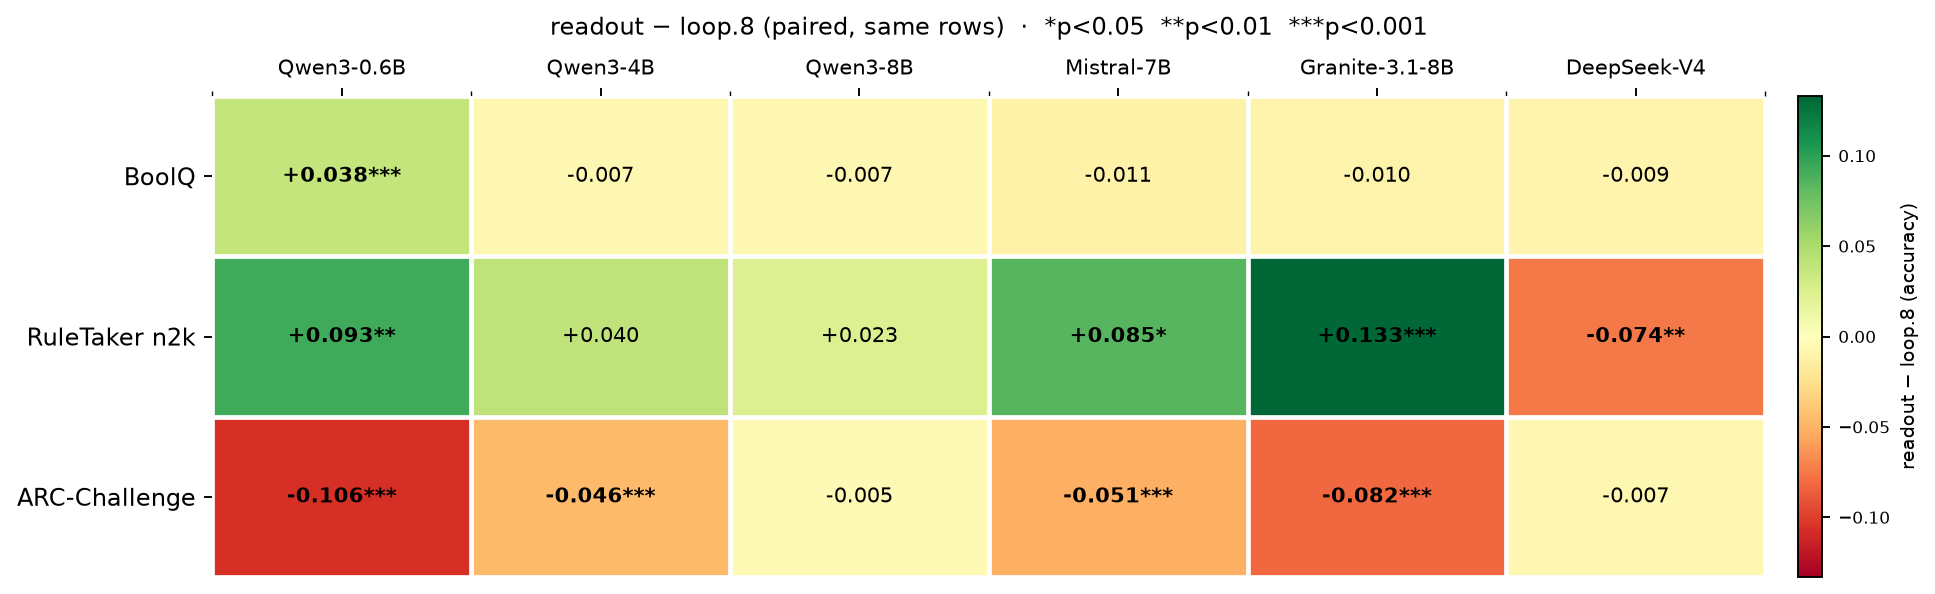
\includegraphics[width=\textwidth]{figures/tasklaw_summary.png}
\caption{\textbf{The task law.} readout $-$ loop.$k$ (paired, same rows) per
task$\times$model cell, with McNemar significance. Green everywhere except two
red corners --- small models on parametric ARC, and the frontier MoE on serial
RuleTaker.}
\label{fig:tasklaw}
\end{figure*}

\begin{figure*}[t]
\centering

\includegraphics[width=\textwidth]{figures/layersweep_placement.png}
\caption{\textbf{Readout probe-placement sweeps} (18 cells). One-pass \head{}
accuracy vs tapped residual layer; loop arms as horizontal references; paired
McNemar annotation per panel. Mid-depth taps win significantly at 9/18 cells
and never lose.}
\label{fig:placement}
\end{figure*}

\begin{figure}[t]
\centering

\includegraphics[width=\columnwidth]{figures/boolq_results.png}
\caption{\textbf{BoolQ: \head{} vs loop} across four scales (full val).}
\label{fig:boolq}
\end{figure}

\begin{figure}[t]
\centering

\includegraphics[width=\columnwidth]{figures/head_to_head_three_tasks.png}
\caption{\textbf{Three-task head-to-head} (BoolQ $\cdot$ RuleTaker $\cdot$
ARC) across models.}
\label{fig:h2h}
\end{figure}

\begin{figure}[t]
\centering
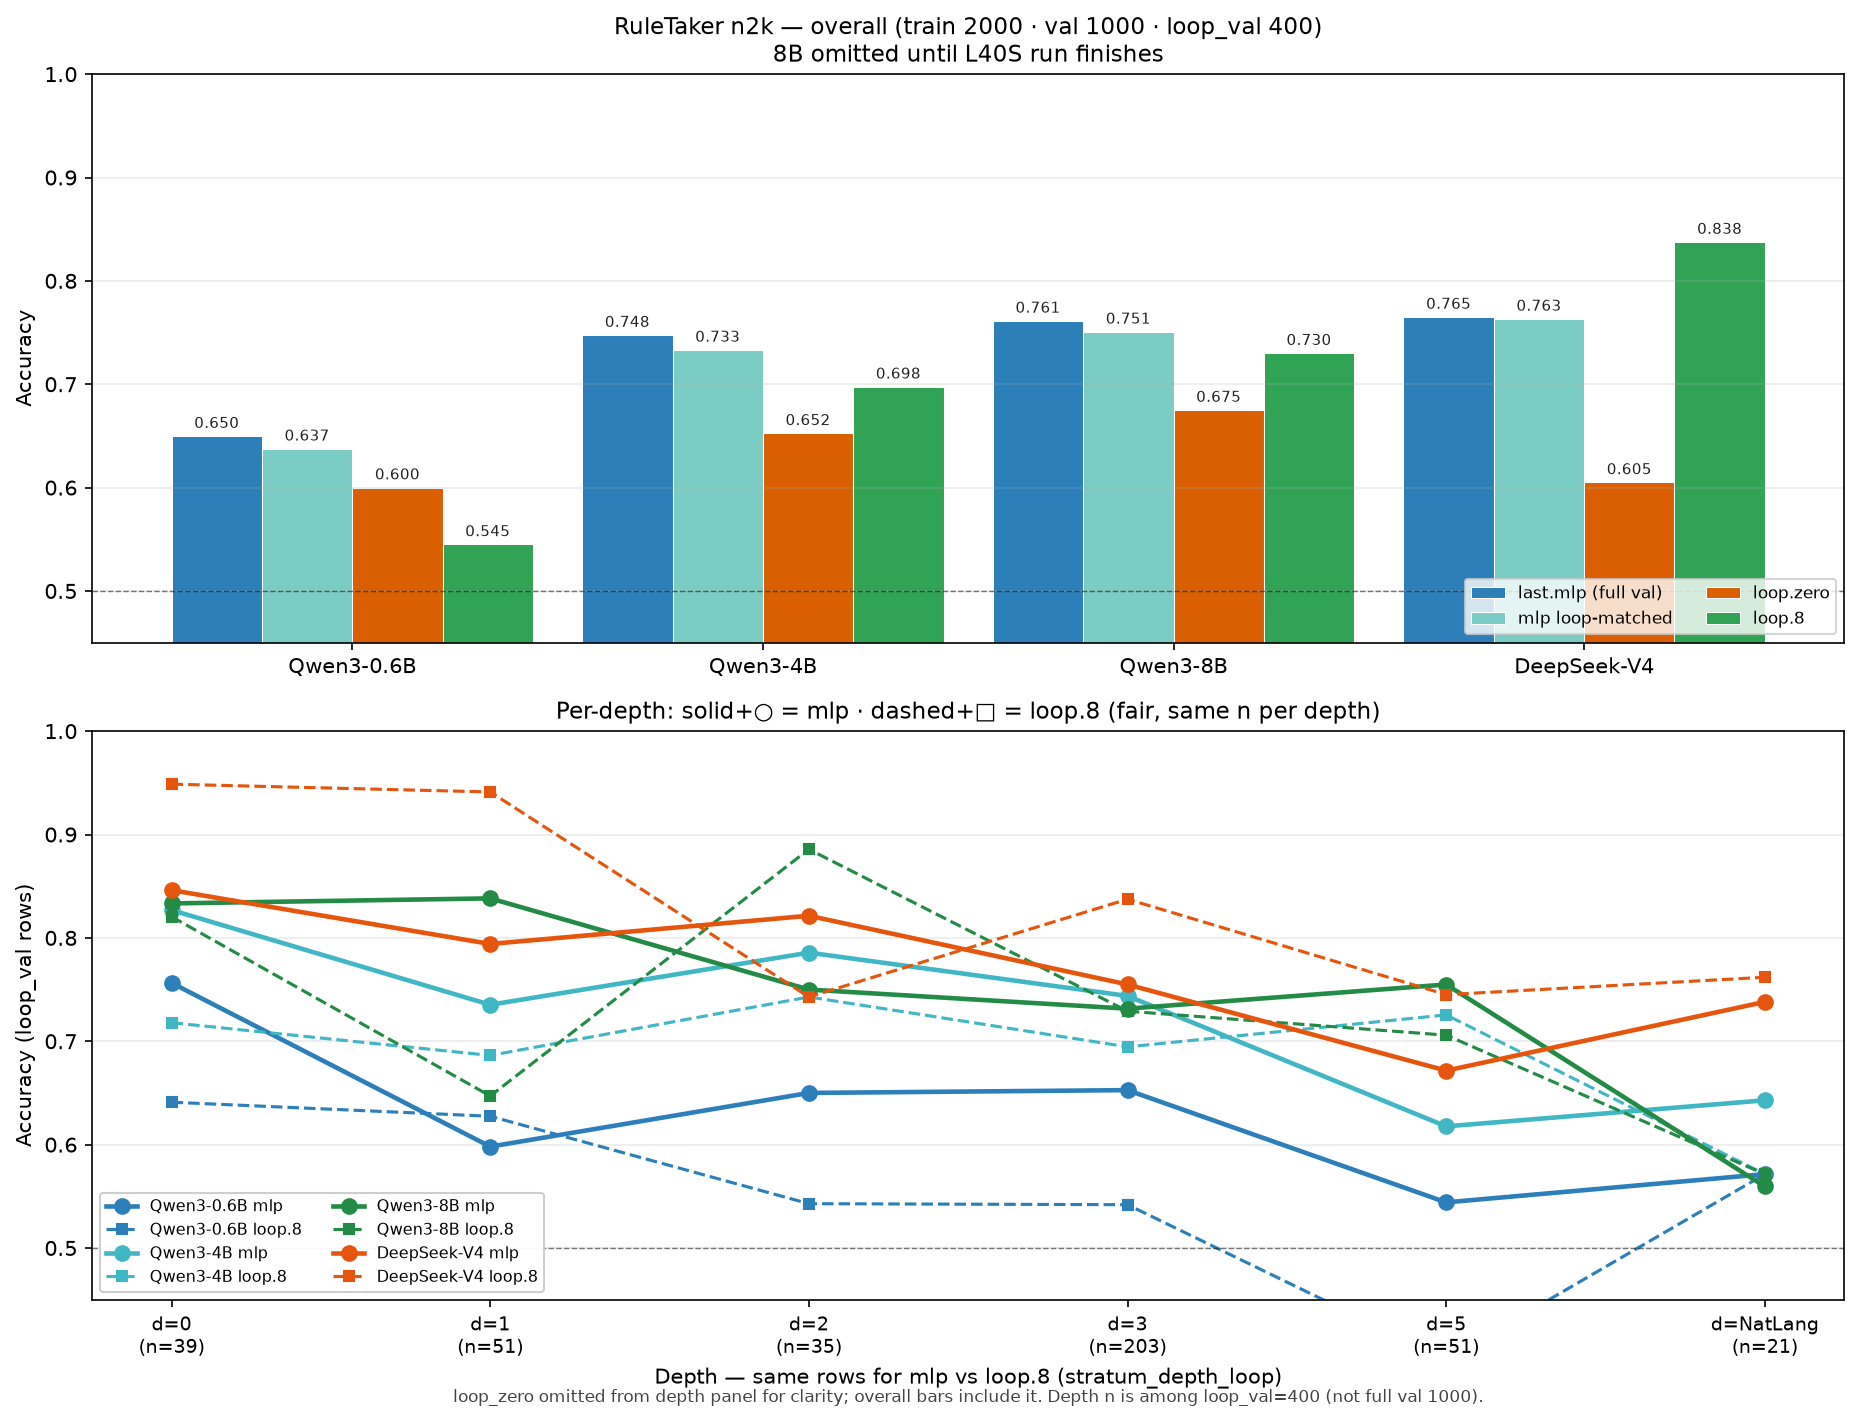
\includegraphics[width=\columnwidth]{figures/ruletaker_depth_strata.png}
\caption{\textbf{RuleTaker overall $+$ per-depth strata}, \head{} vs loop.}
\label{fig:depth}
\end{figure}

\begin{figure}[t]
\centering

\includegraphics[width=\columnwidth]{figures/boolq_budget_kcurve.png}
\caption{\textbf{Supervision budget (Ext 13).} The loop's $k$-curve plateaus
by $k{=}32$ and never passes the \head{}.}
\label{fig:kcurve}
\end{figure}

\begin{figure}[t]
\centering
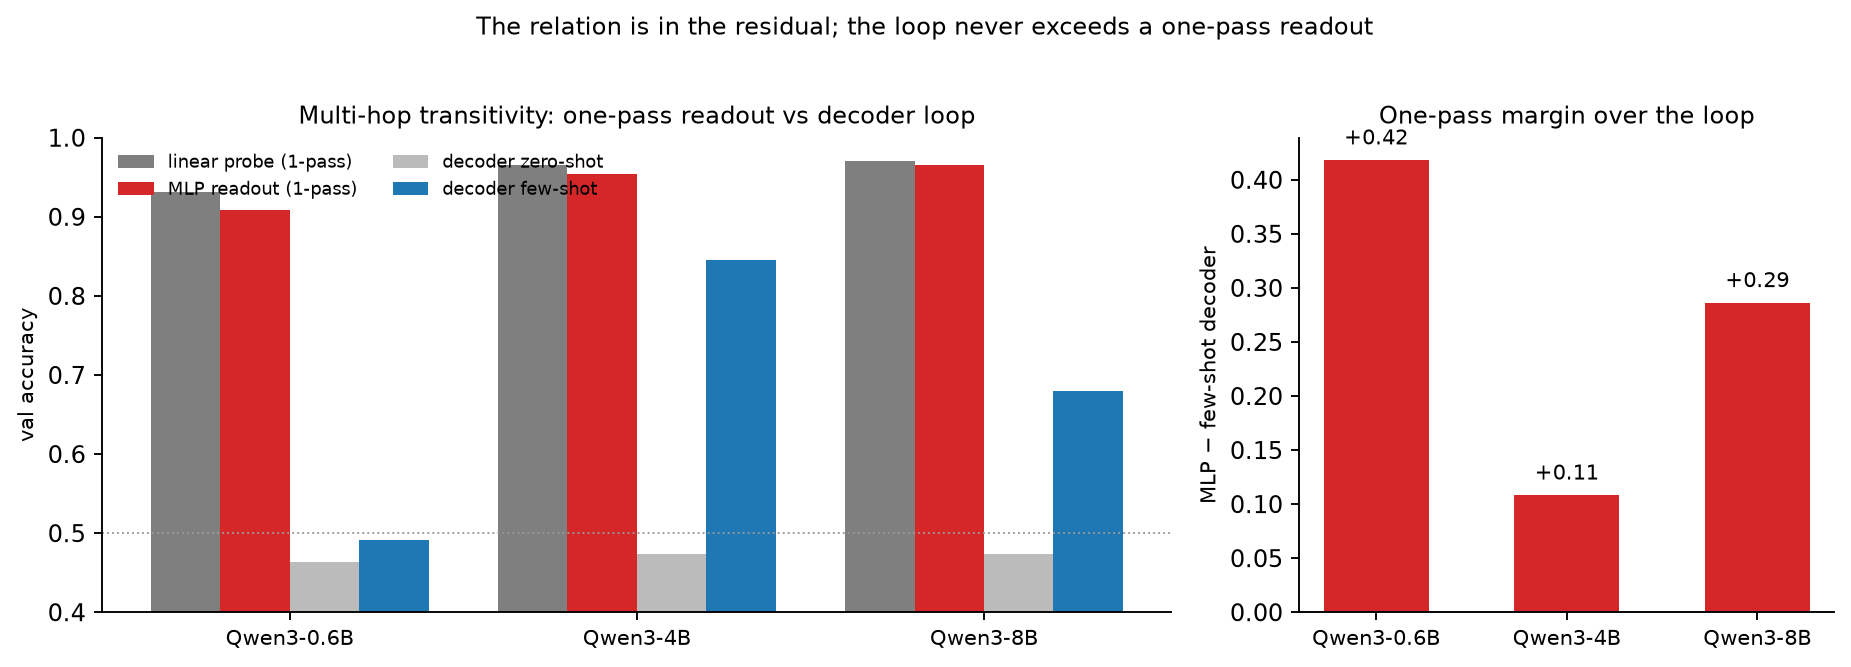
\includegraphics[width=\columnwidth]{figures/synthetic_multihop.png}
\caption{\textbf{Mechanism (synthetic).} Multi-hop transitivity: one-pass
\head{} vs decoder loop across Qwen3 scale. The loop never exceeds a one-pass
\head{}.}
\label{fig:synthetic}
\end{figure}

% ----------------------------------------------------------------- tables --
% Canonical tables, shared by main_tables.tex (standalone) and paper.tex.
% All numbers: post-fix canonicals, batch 8, model-pinned GPUs (2026-08-10/11).
% Requires: booktabs, multirow, caption, graphicx (\resizebox), and
% \sd \pstar \pstarstar \pstarstarstar.
% Shrink-only fit: never upscale a narrow table to \textwidth (that made
% Table~4 look oversized).
\newcommand{\fittable}[1]{%
  \sbox0{#1}%
  \ifdim\wd0>\textwidth
    \resizebox{\textwidth}{!}{\usebox0}%
  \else
    \usebox0
  \fi
}

\begin{table*}[t]
\centering
\caption{\textbf{One-pass residual readout vs.\ fair AR closed-set scorer}
(accuracy). Readout: MLP on frozen final residual (\emph{per-seed mean};
BoolQ/ARC finals match Table~\ref{tab:placement}; RuleTaker is the 10k/4k
run). Loop: next-token log-prob over the closed answer
set, full context, balanced few-shot --- not free-form generation. loop.0 /
loop.8 = zero- / 8-shot; \emph{best loop} = stronger arm ($k$ in
parentheses; RT 0.6B and ARC DSV4 prefer zero-shot). $\Delta=$ readout $-$
best loop (best-of makes $\Delta$ conservative). Paired McNemar on
identical rows using 4-seed vote preds (mean--vote $\le$0.9pt; never flips
sig/ns). Stars mark \emph{uncorrected} $p$
($^{\ast}p{<}0.05$, $^{\ast\ast}p{<}0.01$, $^{\ast\ast\ast}p{<}0.001$);
all 12 raw-significant cells remain significant under Benjamini--Hochberg
FDR at $q{<}0.05$ across the 18 cells.
\textsuperscript{a}BoolQ val 3270; Qwen $k{\le}64$ pad 8192, else $k{=}8$
pad 2048.
\textsuperscript{b}RuleTaker 10k/4k, val 4000 (same rows for readout and
loop). Table~\ref{tab:placement} is a separate layer-sweep; its RuleTaker
finals are not these numbers.
\textsuperscript{c}ARC-Challenge test 1165, $k{=}8$.}
\label{tab:main}
\small
\setlength{\tabcolsep}{3.5pt}%
\fittable{%
\begin{tabular}{@{}llcccccc@{}}
\toprule
Task & Model & Readout & loop.0 & loop.8 & best loop & $\Delta$ (readout $-$ loop) & $p$ (McNemar) \\
\midrule
\multirow{6}{*}{BoolQ\textsuperscript{a}}
 & Qwen3-0.6B & \textbf{0.746} & 0.631 & 0.645 & 0.715\,(32) & \sd{+0.030}\pstarstarstar & $3.2\mathrm{e}{-05}$ \\
 & Qwen3-4B   & 0.856 & 0.855 & 0.865 & \textbf{0.867}\,(64) & $-0.012$ & 0.094 \\
 & Qwen3-8B   & 0.878 & 0.862 & 0.876 & \textbf{0.886}\,(16) & $-0.008$ & 0.243 \\
 & Mistral-7B & 0.841 & 0.824 & 0.863 & \textbf{0.863}\,(8) & \sd{$-0.022$}\pstarstar & 0.003 \\
 & Granite-3.1-8B & 0.854 & 0.800 & 0.865 & \textbf{0.865}\,(8) & $-0.011$ & 0.076 \\
 & DeepSeek-V4-Flash & 0.896 & 0.888 & 0.906 & \textbf{0.906}\,(8) & $-0.009$ & 0.078 \\
\midrule
\multirow{6}{*}{RuleTaker\textsuperscript{b}}
 & Qwen3-0.6B & \textbf{0.684} & 0.593 & 0.580 & 0.593\,(zero) & \sd{+0.090}\pstarstarstar & $1.0\mathrm{e}{-20}$ \\
 & Qwen3-4B   & \textbf{0.782} & 0.678 & 0.690 & 0.690\,(8) & \sd{+0.092}\pstarstarstar & $6.8\mathrm{e}{-29}$ \\
 & Qwen3-8B   & \textbf{0.782} & 0.678 & 0.736 & 0.736\,(8) & \sd{+0.046}\pstarstarstar & $1.6\mathrm{e}{-09}$ \\
 & Mistral-7B & \textbf{0.682} & 0.522 & 0.571 & 0.571\,(8) & \sd{+0.111}\pstarstarstar & $4.2\mathrm{e}{-28}$ \\
 & Granite-3.1-8B & \textbf{0.823} & 0.564 & 0.703 & 0.703\,(8) & \sd{+0.119}\pstarstarstar & $1.1\mathrm{e}{-45}$ \\
 & DeepSeek-V4-Flash & 0.797 & 0.600 & 0.813 & \textbf{0.813}\,(8) & \sd{$-0.016$}\pstar & 0.029 \\
\midrule
\multirow{6}{*}{ARC-Challenge\textsuperscript{c}}
 & Qwen3-0.6B & 0.492 & 0.502 & 0.597 & \textbf{0.597}\,(8) & \sd{$-0.106$}\pstarstarstar & $3.2\mathrm{e}{-11}$ \\
 & Qwen3-4B   & 0.841 & 0.826 & 0.882 & \textbf{0.882}\,(8) & \sd{$-0.041$}\pstarstarstar & $2.9\mathrm{e}{-06}$ \\
 & Qwen3-8B   & 0.909 & 0.902 & 0.913 & \textbf{0.913}\,(8) & $-0.004$ & 0.567 \\
 & Mistral-7B & 0.728 & 0.750 & 0.779 & \textbf{0.779}\,(8) & \sd{$-0.051$}\pstarstarstar & $9.3\mathrm{e}{-05}$ \\
 & Granite-3.1-8B & 0.708 & 0.732 & 0.790 & \textbf{0.790}\,(8) & \sd{$-0.082$}\pstarstarstar & $5.8\mathrm{e}{-10}$ \\
 & DeepSeek-V4-Flash & 0.951 & 0.961 & 0.959 & \textbf{0.961}\,(zero) & $-0.010$ & 0.064 \\
\bottomrule
\end{tabular}%
}
\end{table*}

\begin{table*}[t]
\centering
\caption{\textbf{Readout probe-placement sweeps} (18 cells, all batch 8):
best mid-depth tap vs the final-layer readout. $\Delta=$ displayed best $-$
displayed final (per-seed means). $p$ is paired McNemar on 4-seed vote
(mean--vote can differ by ${\sim}$1pt). RuleTaker finals are this layer-sweep,
not Table~\ref{tab:main}. \emph{Layers} = stack depth
(28/36/36/32/40/43). \emph{Plateau onset} = first swept layer within
1\,pt of the final-layer readout --- a lightweight readout extracts nearly as
much label information from there on as from the final residual; at
DeepSeek-V4 this happens by L22/42 (52\% depth)
on \emph{all three tasks}, with ARC showing the sharpest snap-in
(near-chance at L15 $\to$ 0.944 at L22). This is representation sufficiency,
not a claim that later layers can be skipped. Mid-depth taps win significantly at
9/18 cells raw (6/18 after Benjamini--Hochberg FDR at $q{<}0.05$) and never
lose significantly.}
\label{tab:placement}
\small
\setlength{\tabcolsep}{3.5pt}%
\fittable{%
\begin{tabular}{@{}llcccccccc@{}}
\toprule
Task & Model & \# & Tap & Dep. & Plateau & best & final & $\Delta$ & $p$ \\
\midrule
\multirow{6}{*}{BoolQ}
  & Qwen3-0.6B & 28 & L18 & 64\% & L18 (67\%) &0.761 & 0.746 & $+0.015$ & 0.18 \\
  & Qwen3-4B   & 36 & L24 & 67\% & L24 (69\%) &0.868 & 0.856 & \sd{+0.012}\pstar & 0.038 \\
  & Qwen3-8B   & 36 & L30 & 83\% & L24 (69\%) &0.889 & 0.878 & \sd{+0.011}\pstar & 0.016 \\
  & Mistral-7B & 32 & L16 & 50\% & \sd{L16 (52\%)} &0.863 & 0.841 & \sd{+0.022}\pstarstarstar & $1.1\mathrm{e}{-04}$ \\
  & Granite-3.1-8B & 40 & L20 & 51\% & \sd{L17 (44\%)} &0.868 & 0.854 & \sd{+0.014}\pstarstar & $1.0\mathrm{e}{-03}$ \\
  & DeepSeek-V4-Flash & 43 & L36 & 86\% & \sd{L22 (52\%)} &0.900 & 0.896 & $+0.004$ & 0.20 \\
\midrule
\multirow{6}{*}{RuleTaker}
  & Qwen3-0.6B & 28 & L18 & 64\% & \sd{L13 (48\%)} &0.688 & 0.650 & \sd{+0.038}\pstar & 0.020 \\
  & Qwen3-4B   & 36 & L24 & 67\% & L24 (69\%) &0.781 & 0.744 & \sd{+0.037}\pstarstar & $2.8\mathrm{e}{-03}$ \\
  & Qwen3-8B   & 36 & L24 & 67\% & L24 (69\%) &0.778 & 0.758 & \sd{+0.020}\pstar & 0.040 \\
  & Mistral-7B & 32 & L18 & 56\% & \sd{L11 (35\%)} &0.702 & 0.643 & \sd{+0.059}\pstarstarstar & $5.2\mathrm{e}{-05}$ \\
  & Granite-3.1-8B & 40 & L20 & 51\% & L20 (51\%) &0.816 & 0.805 & $+0.011$ & 0.37 \\
  & DeepSeek-V4-Flash & 43 & L29 & 67\% & \sd{L22 (52\%)} &0.776 & 0.765 & $+0.011$ & 0.057 \\
\midrule
\multirow{6}{*}{ARC-Challenge}
  & Qwen3-0.6B & 28 & L26 & 93\% & L26 (96\%) &0.500 & 0.492 & $+0.008$ & 0.082 \\
  & Qwen3-4B   & 36 & L29 & 81\% & L24 (69\%) &0.856 & 0.841 & \sd{+0.015}\pstarstarstar & $2.2\mathrm{e}{-04}$ \\
  & Qwen3-8B   & 36 & L35 & 97\% & L24 (69\%) &0.909 & 0.909 & $0.000$ & 1.00 \\
  & Mistral-7B & 32 & L20 & 63\% & L18 (58\%) &0.741 & 0.728 & $+0.013$ & 0.50 \\
  & Granite-3.1-8B & 40 & L39 & 100\% & L39 (100\%) &0.708 & 0.708 & $0.000$ & --- \\
  & DeepSeek-V4-Flash & 43 & L42 & 98\% & \sd{L22 (52\%)} &0.951 & 0.951 & $0.000$ & --- \\
\bottomrule
\end{tabular}%
}
\end{table*}


\begin{table*}[t]
\centering
\caption{\textbf{Controls, all 18 cells.} Every headline number clears all
four controls. \emph{label-shuffle}: the head refit on permuted labels sits at
chance. \emph{random-projection}: a head on random Gaussian projections
retains accuracy with permuted-basis $\approx$ max-basis $\gg$ noise floor ---
the signal is \emph{diffuse}. \emph{full-context}: a mean-pooled full-context
readout underperforms the final-token readout --- the verdict is computed into
the final state, not read off the passage. Balanced chance is 0.50 (BoolQ,
RuleTaker) and 0.25 (4-way ARC); the \emph{majority-class} baseline is
$\approx$0.62 (BoolQ), 0.50 (RuleTaker), 0.27 (ARC).}
\label{tab:controls}
\small
\setlength{\tabcolsep}{4pt}%
\begin{tabular}{@{}llcccccc@{}}
\toprule
Task & Model & shuffle & rp max & rp perm & rp noise & full-ctx & final \\
\midrule
\multirow{6}{*}{BoolQ}
  & Qwen3-0.6B & 0.533 & 0.734 & 0.725 & 0.601 & 0.667 & 0.746 \\
  & Qwen3-4B & 0.542 & 0.861 & 0.859 & 0.604 & 0.717 & 0.856 \\
  & Qwen3-8B & 0.528 & 0.874 & 0.874 & 0.607 & 0.739 & 0.878 \\
  & Mistral-7B & 0.537 & 0.810 & 0.803 & 0.607 & 0.685 & 0.841 \\
  & Granite-3.1-8B & 0.532 & 0.848 & 0.849 & 0.607 & 0.679 & 0.854 \\
  & DeepSeek-V4 & 0.522 & 0.889 & 0.891 & 0.602 & 0.678 & 0.896 \\
\midrule
\multirow{6}{*}{RuleTaker}
  & Qwen3-0.6B & 0.498 & 0.657 & 0.663 & 0.502 & 0.532 & 0.684 \\
  & Qwen3-4B & 0.516 & 0.748 & 0.752 & 0.490 & 0.619 & 0.782 \\
  & Qwen3-8B & 0.506 & 0.760 & 0.755 & 0.502 & 0.634 & 0.782 \\
  & Mistral-7B & 0.503 & 0.656 & 0.646 & 0.502 & 0.521 & 0.682 \\
  & Granite-3.1-8B & 0.504 & 0.792 & 0.785 & 0.502 & 0.599 & 0.823 \\
  & DeepSeek-V4 & 0.509 & 0.768 & 0.759 & 0.503 & 0.526 & 0.797 \\
\midrule
\multirow{6}{*}{ARC}
  & Qwen3-0.6B & 0.278 & 0.470 & 0.470 & 0.254 & 0.278 & 0.492 \\
  & Qwen3-4B & 0.269 & 0.802 & 0.803 & 0.255 & 0.349 & 0.841 \\
  & Qwen3-8B & 0.287 & 0.869 & 0.867 & 0.251 & 0.399 & 0.909 \\
  & Mistral-7B & 0.259 & 0.679 & 0.678 & 0.251 & 0.277 & 0.728 \\
  & Granite-3.1-8B & 0.284 & 0.598 & 0.588 & 0.251 & 0.279 & 0.708 \\
  & DeepSeek-V4 & 0.269 & 0.942 & 0.940 & 0.236 & 0.439 & 0.951 \\
\bottomrule
\end{tabular}
\end{table*}


\end{document}
